\documentclass[aspectratio=169]{beamer}
\usepackage[utf8]{inputenc}
\usepackage{lmodern}
\usepackage{tikz}
\usepackage{hyperref}
\hypersetup{hidelinks}
\usetikzlibrary{positioning,arrows.meta,calc}

\definecolor{accent1}{HTML}{0F766E}
\definecolor{accent2}{HTML}{99F6E4}
\definecolor{accent3}{HTML}{F59E0B}
\definecolor{accent4}{HTML}{134E4A}
\definecolor{paper}{HTML}{F7FEFC}
\definecolor{ink}{HTML}{1F2937}

\newcommand{\PromptCopyBase}{lesson1-prompt-cards-copy.html}
\newcommand{\PromptLink}[2]{\href{\PromptCopyBase\##1}{#2}}
\newcommand{\CopyChip}[1]{%
	\href{\PromptCopyBase\##1}{%
		\tikz[baseline=-0.6ex] \node[
			rounded corners=6pt,
			fill=accent2!24,
			draw=accent1!80!black,
			line width=0.6pt,
			inner xsep=6pt,
			inner ysep=2.2pt
		]{\scriptsize\bfseries Copy};%
	}%
}

\setbeamertemplate{navigation symbols}{}
\setbeamercolor{normal text}{fg=ink,bg=white}
\setbeamercolor{frametitle}{fg=ink,bg=white}
\setbeamertemplate{itemize item}{\color{accent1}$\blacktriangleright$}
\setbeamertemplate{enumerate item}{\color{accent1}\insertenumlabel.}
\setbeameroption{hide notes}

\title{Lesson 1: Brainstorm and Plan}
\subtitle{MagicSchool Student Project Guide}
\author{Pine Brook IGNITE}
\date{Spring 2026}

\begin{document}

\begin{frame}[plain]
\begin{tikzpicture}[remember picture,overlay]
\fill[paper] (current page.south west) rectangle (current page.north east);
\fill[accent1!10] (0.25,0.4) rectangle (13.05,7.0);
\draw[line width=7pt, color=accent3] (0.55,6.75) -- (12.75,6.75);
\draw[line width=7pt, color=accent2] (0.55,0.65) -- (12.75,0.65);
\end{tikzpicture}
\vspace{0.45cm}
\begin{columns}[T,totalwidth=\textwidth]
\column{0.57\textwidth}
{\huge\bfseries\color{ink} Lesson 1: Brainstorm and Plan\par}
\vspace{0.2cm}
{\Large\color{accent4} Pick a topic. Check it. Plan it.\par}
\vspace{0.25cm}

\begin{tikzpicture}
\node[rounded corners=16pt, fill=white, draw=accent1, line width=1.2pt, text width=6.4cm, minimum height=1.35cm, align=center]
{\Large\bfseries AI helps us think. We stay in charge.};
\end{tikzpicture}
\vspace{0.35cm}
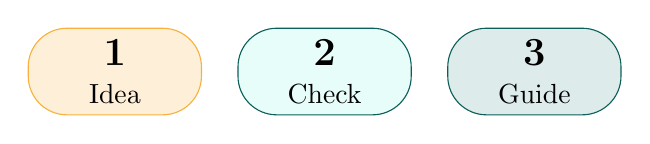
\begin{tikzpicture}[node distance=0.45cm]
\node[rounded corners=14pt, fill=accent3!16, draw=accent3!80, minimum width=2.2cm, minimum height=1.1cm, align=center] (a) {\Large\bfseries 1\\[2pt]Idea};
\node[rounded corners=14pt, fill=accent2!24, draw=accent1!80!black, minimum width=2.2cm, minimum height=1.1cm, align=center, right=of a] (b) {\Large\bfseries 2\\[2pt]Check};
\node[rounded corners=14pt, fill=accent1!14, draw=accent1!80!black, minimum width=2.2cm, minimum height=1.1cm, align=center, right=of b] (c) {\Large\bfseries 3\\[2pt]Guide};
\end{tikzpicture}
\column{0.38\textwidth}
\begin{center}
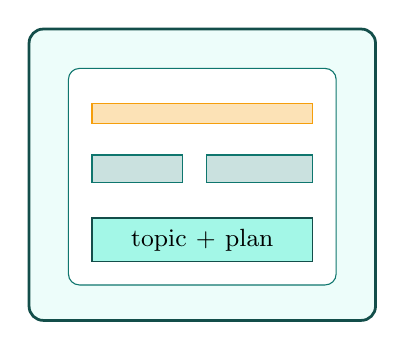
\begin{tikzpicture}[x=1cm,y=1cm]
\draw[rounded corners=0.18cm, fill=accent2!18, draw=accent4, line width=1pt] (0.4,0.5) rectangle (4.8,4.2);
\draw[rounded corners=0.14cm, fill=white, draw=accent1] (0.9,0.95) rectangle (4.3,3.7);
\draw[fill=accent3!30, draw=accent3] (1.2,3.0) rectangle (4.0,3.25);
\draw[fill=accent1!22, draw=accent1] (1.2,2.25) rectangle (2.35,2.6);
\draw[fill=accent1!22, draw=accent1] (2.65,2.25) rectangle (4.0,2.6);
\draw[fill=accent2!90, draw=accent4] (1.2,1.25) rectangle (4.0,1.8);
\node[text width=2.3cm, align=center] at (2.6,1.52) {\small topic + plan};
\end{tikzpicture}
\end{center}
\end{columns}
\note{Open with the mission: by the end of class students have a topic, a CS connection, and a high-level guide.}
\end{frame}

\begin{frame}[plain]
\frametitle{Today's Mission}
\begin{block}{By the end of Lesson 1, I will have:}
\begin{itemize}
\large
\item one topic I care about
\item one reason it connects to computer science
\item one project type
\item a guide with 3 to 5 parts, sections, or questions
\end{itemize}
\end{block}
\vspace{0.15cm}
\begin{center}
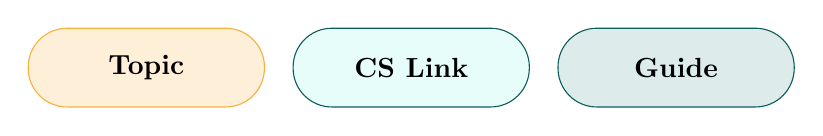
\begin{tikzpicture}[node distance=0.35cm]
\node[rounded corners=14pt, fill=accent3!16, draw=accent3!80, minimum width=3.0cm, minimum height=1.0cm, align=center] (a) {\bfseries Topic};
\node[rounded corners=14pt, fill=accent2!24, draw=accent1!80!black, minimum width=3.0cm, minimum height=1.0cm, align=center, right=of a] (b) {\bfseries CS Link};
\node[rounded corners=14pt, fill=accent1!14, draw=accent1!80!black, minimum width=3.0cm, minimum height=1.0cm, align=center, right=of b] (c) {\bfseries Guide};
\end{tikzpicture}
\end{center}
\note{Keep success criteria visible.}
\end{frame}

\begin{frame}[plain]
\frametitle{Our AI Rules}
\begin{columns}[T,totalwidth=\textwidth]
\column{0.54\textwidth}
\begin{itemize}
\large
\item Do not type names or private information.
\item AI is a helper, not the boss.
\item AI can be wrong.
\item We choose what to keep or change.
\item The teacher can see class AI work.
\end{itemize}
\column{0.4\textwidth}
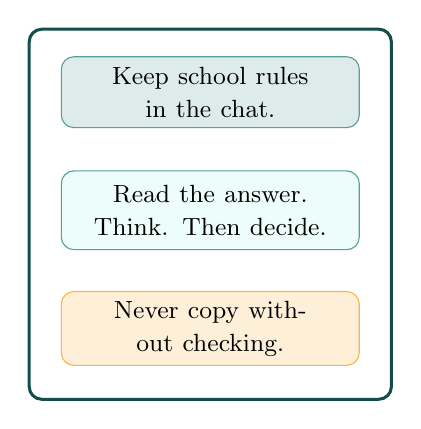
\begin{tikzpicture}[x=1cm,y=1cm]
\draw[rounded corners=0.16cm, fill=white, draw=accent4, line width=1.1pt] (0.1,0.1) rectangle (4.7,4.8);
\node[rounded corners=0.16cm, fill=accent1!14, draw=accent1!70, text width=3.55cm, minimum height=0.9cm, align=center] at (2.4,4.0) {\small Keep school rules in the chat.};
\node[rounded corners=0.16cm, fill=accent2!18, draw=accent1!70, text width=3.55cm, minimum height=1.0cm, align=center] at (2.4,2.5) {\small Read the answer. Think. Then decide.};
\node[rounded corners=0.16cm, fill=accent3!16, draw=accent3!75, text width=3.55cm, minimum height=0.9cm, align=center] at (2.4,1.0) {\small Never copy without checking.};
\end{tikzpicture}
\end{columns}
\note{Name safety expectations before devices open.}
\end{frame}

\begin{frame}[plain]
\frametitle{Use the Right Tool}
\begin{columns}[T,totalwidth=\textwidth]
\column{0.48\textwidth}
\begin{block}{Idea Generator}
\begin{itemize}
\large
\item Start here
\item Get possible topic ideas
\item Connect your interests to CS
\end{itemize}
\end{block}
\column{0.48\textwidth}
\begin{block}{AI Assistant}
\begin{itemize}
\large
\item Use after you have an idea
\item Check the CS connection
\item Make the topic smaller
\item Build a guide with 3 to 5 parts
\end{itemize}
\end{block}
\end{columns}
\vspace{0.15cm}
\begin{center}
\Large\bfseries Idea Generator first. AI Assistant second.
\end{center}
\note{This slide is the main tool-separation scaffold.}
\end{frame}

\begin{frame}[plain]
\frametitle{Our Workflow}
\begin{center}
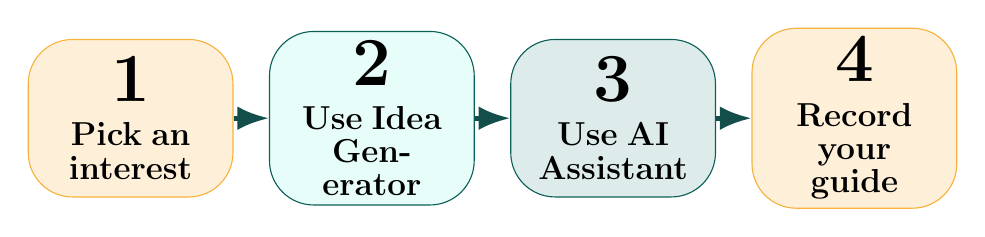
\begin{tikzpicture}[node distance=0.45cm]
\node[rounded corners=16pt, fill=accent3!16, draw=accent3!80, minimum width=2.6cm, minimum height=2.0cm, text width=2.0cm, align=center] (s1) {\Huge\bfseries 1\\[4pt]\large Pick an interest};
\node[rounded corners=16pt, fill=accent2!24, draw=accent1!80!black, minimum width=2.6cm, minimum height=2.0cm, text width=2.0cm, align=center, right=of s1] (s2) {\Huge\bfseries 2\\[4pt]\large Use Idea Generator};
\node[rounded corners=16pt, fill=accent1!14, draw=accent1!80!black, minimum width=2.6cm, minimum height=2.0cm, text width=2.0cm, align=center, right=of s2] (s3) {\Huge\bfseries 3\\[4pt]\large Use AI Assistant};
\node[rounded corners=16pt, fill=accent3!16, draw=accent3!80, minimum width=2.6cm, minimum height=2.0cm, text width=2.0cm, align=center, right=of s3] (s4) {\Huge\bfseries 4\\[4pt]\large Record your guide};
\draw[-{Latex[length=4mm,width=3mm]}, line width=1.7pt, color=accent4] (s1) -- (s2);
\draw[-{Latex[length=4mm,width=3mm]}, line width=1.7pt, color=accent4] (s2) -- (s3);
\draw[-{Latex[length=4mm,width=3mm]}, line width=1.7pt, color=accent4] (s3) -- (s4);
\end{tikzpicture}
\end{center}
\vspace{0.25cm}
\begin{block}{Remember}
\large You do not need a finished project today. You need a strong topic and a strong guide.
\end{block}
\note{Helps students separate planning from building.}
\end{frame}

\begin{frame}[plain]
\frametitle{Prompt Cards: Idea Generator}
\begin{block}{Use Idea Generator for topic ideas}
\begin{itemize}
\large
\item \CopyChip{ig1}\hspace{0.6em}\PromptLink{ig1}{My interest is \_\_\_\_. Give me 4 computer-science project ideas for grades 4-5.}
\item \CopyChip{ig2}\hspace{0.6em}\PromptLink{ig2}{Help me turn my interest in \_\_\_\_ into a computer-science project topic.}
% \item Give me 4 project topic ideas that connect \_\_\_\_, technology, and computer science.
\end{itemize}
\end{block}
\vspace{0.2cm}
\begin{center}
\Large\bfseries Pick 1 or 2 ideas worth checking.
\end{center}
\note{Project this while students use Idea Generator.}
\end{frame}

\begin{frame}[plain]
\frametitle{Prompt Cards: AI Assistant}
\begin{block}{Use AI Assistant for checking and planning}
\begin{itemize}
\large
\item \CopyChip{aa1}\hspace{0.6em}\PromptLink{aa1}{My topic is \_\_\_\_. Is this really connected to computer science? Explain how.}
\item \CopyChip{aa2}\hspace{0.6em}\PromptLink{aa2}{My topic is \_\_\_\_. Help me make it smaller and clearer for a short project.}
\item \CopyChip{aa3}\hspace{0.6em}\PromptLink{aa3}{My topic is \_\_\_\_. Give me a high-level guide with 3 to 5 parts, sections, or questions I could use for my project.}
\end{itemize}
\end{block}
\vspace{0.2cm}
\begin{center}
\Large\bfseries Choose a guide you agree with.
\end{center}
\note{Project this while students use AI Assistant.}
\end{frame}

\begin{frame}[plain]
\frametitle{What Not To Do}
\begin{columns}[T,totalwidth=\textwidth]
\column{0.48\textwidth}
\begin{block}{Do}
\begin{itemize}
\large
\item read the answer
\item check if it fits your goal
\item pick the parts you agree with
\item ask for a better version if needed
\end{itemize}
\end{block}
\column{0.52\textwidth}
\begin{block}{Do Not}
\begin{itemize}
\large
\item just copy the whole answer
\item accept the first answer right away
\item keep a topic that is too long/complex
\item choose a topic with no CS connection
\end{itemize}
\end{block}
\end{columns}
\note{Explicitly model what not to do.}
\end{frame}

\begin{frame}[plain]
\frametitle{What Goes on Your Planning Sheet?}
\begin{itemize}
\large
\item My topic:
\item My CS connection:
\item My project type:
\item My guide with 3 to 5 parts, sections, or questions:
\end{itemize}
\vspace{0.18cm}
\begin{block}{Optional AI helper (click Copy)}
\small \CopyChip{ps1}\hspace{0.6em}\PromptLink{ps1}{My topic is \_\_\_\_. My interest is \_\_\_\_. Help me fill out my planning sheet in the right format.}
\end{block}
\vspace{0.12cm}
\begin{block}{Teacher check}
\Large Before Lesson 2, your topic and guide must be approved.
\end{block}
\note{Keep this visible during record time.}
\end{frame}

\begin{frame}[plain]
\frametitle{If You Get Stuck}
\begin{columns}[T,totalwidth=\textwidth]
\column{0.56\textwidth}
\begin{block}{Troubleshoot in order}
\begin{enumerate}
\large
\item Name the problem.
\item Try one small change.
\item Use the matching prompt.
\item Read the answer. Keep only what helps you.
\item Ask your partner or teacher.
\end{enumerate}
\end{block}
\column{0.4\textwidth}
\begin{block}{Problem key}
\small
\begin{itemize}
\item \fcolorbox{accent3!75}{accent3!16}{\strut\textbf{No topic yet}}
\item \fcolorbox{accent1!80!black}{accent1!14}{\strut\textbf{Too big}}
\item \fcolorbox{accent2!90!black}{accent2!18}{\strut\textbf{Too simple}}
\item \fcolorbox{accent4}{accent2!10}{\strut\textbf{Don\textquotesingle t like ideas}}
\item \fcolorbox{accent1!80!black}{accent2!24}{\strut\textbf{Not sure it is CS}}
\end{itemize}
\end{block}
\end{columns}
\note{Support without taking over.}
\end{frame}

\begin{frame}[plain]
\frametitle{If You Get Stuck: Copy-Paste Prompts}
\begin{block}{Click Copy, then paste}
\footnotesize
\begin{itemize}
\item \fcolorbox{accent3!75}{accent3!16}{\strut\textbf{No topic yet}} \CopyChip{ts1}\hspace{0.4em}\PromptLink{ts1}{Interests \textrightarrow{} topic ideas}\hspace{0.9em}\CopyChip{ts2}\hspace{0.4em}\PromptLink{ts2}{Questions \textrightarrow{} topic ideas}\\[-1pt]
{\scriptsize Example: \textit{music} \textrightarrow{} a quiz that matches songs to moods}
\item \fcolorbox{accent1!80!black}{accent1!14}{\strut\textbf{Too big}} \CopyChip{ts3}\hspace{0.4em}\PromptLink{ts3}{My topic is \_\_\_\_. Help me make it smaller.}\\[-1pt]
{\scriptsize Example: \textit{animals} \textrightarrow{} one animal + one question + one audience}
\item \fcolorbox{accent2!90!black}{accent2!18}{\strut\textbf{Too simple}} \CopyChip{ts4}\hspace{0.4em}\PromptLink{ts4}{My topic is \_\_\_\_. Help me make it more interesting.}\\[-1pt]
{\scriptsize Example: \textit{soccer} \textrightarrow{} compare positions + make a matching game}
\item \fcolorbox{accent4}{accent2!10}{\strut\textbf{Don\textquotesingle t like ideas}} \CopyChip{ts5}\hspace{0.4em}\PromptLink{ts5}{I do not like these ideas: \_\_\_\_. Give new ones.}
\item \fcolorbox{accent1!80!black}{accent2!24}{\strut\textbf{Not sure it is CS}} \CopyChip{aa1}\hspace{0.4em}\PromptLink{aa1}{My topic is \_\_\_\_. Is this connected to CS?}
\end{itemize}
\end{block}
\note{Use this slide for copy-paste troubleshooting prompts.}
\end{frame}

\begin{frame}[plain]
\frametitle{Ready for Lesson 2?}
\begin{center}
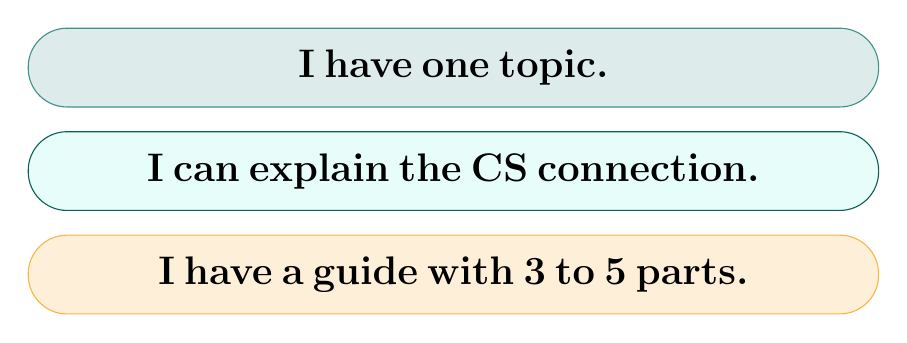
\begin{tikzpicture}[node distance=0.3cm]
\node[rounded corners=14pt, fill=accent1!14, draw=accent1!80, minimum width=10.8cm, minimum height=1.0cm, text width=9.7cm, align=center] (a) {\Large\bfseries I have one topic.};
\node[rounded corners=14pt, fill=accent2!24, draw=accent1!80!black, minimum width=10.8cm, minimum height=1.0cm, text width=9.7cm, align=center, below=of a] (b) {\Large\bfseries I can explain the CS connection.};
\node[rounded corners=14pt, fill=accent3!16, draw=accent3!75, minimum width=10.8cm, minimum height=1.0cm, text width=9.7cm, align=center, below=of b] (c) {\Large\bfseries I have a guide with 3 to 5 parts.};
\end{tikzpicture}
\end{center}
\vspace{0.25cm}
\begin{block}{Quick share}
\Large My topic is\ldots\ My project will be\ldots\ My guide will help me by\ldots
\end{block}
\note{Use as closure and proof of learning.}
\end{frame}

\end{document}
